\begin{figure}[h]
 \centering
 \begin{minipage}[b]{0.32\textwidth}
    \centering
    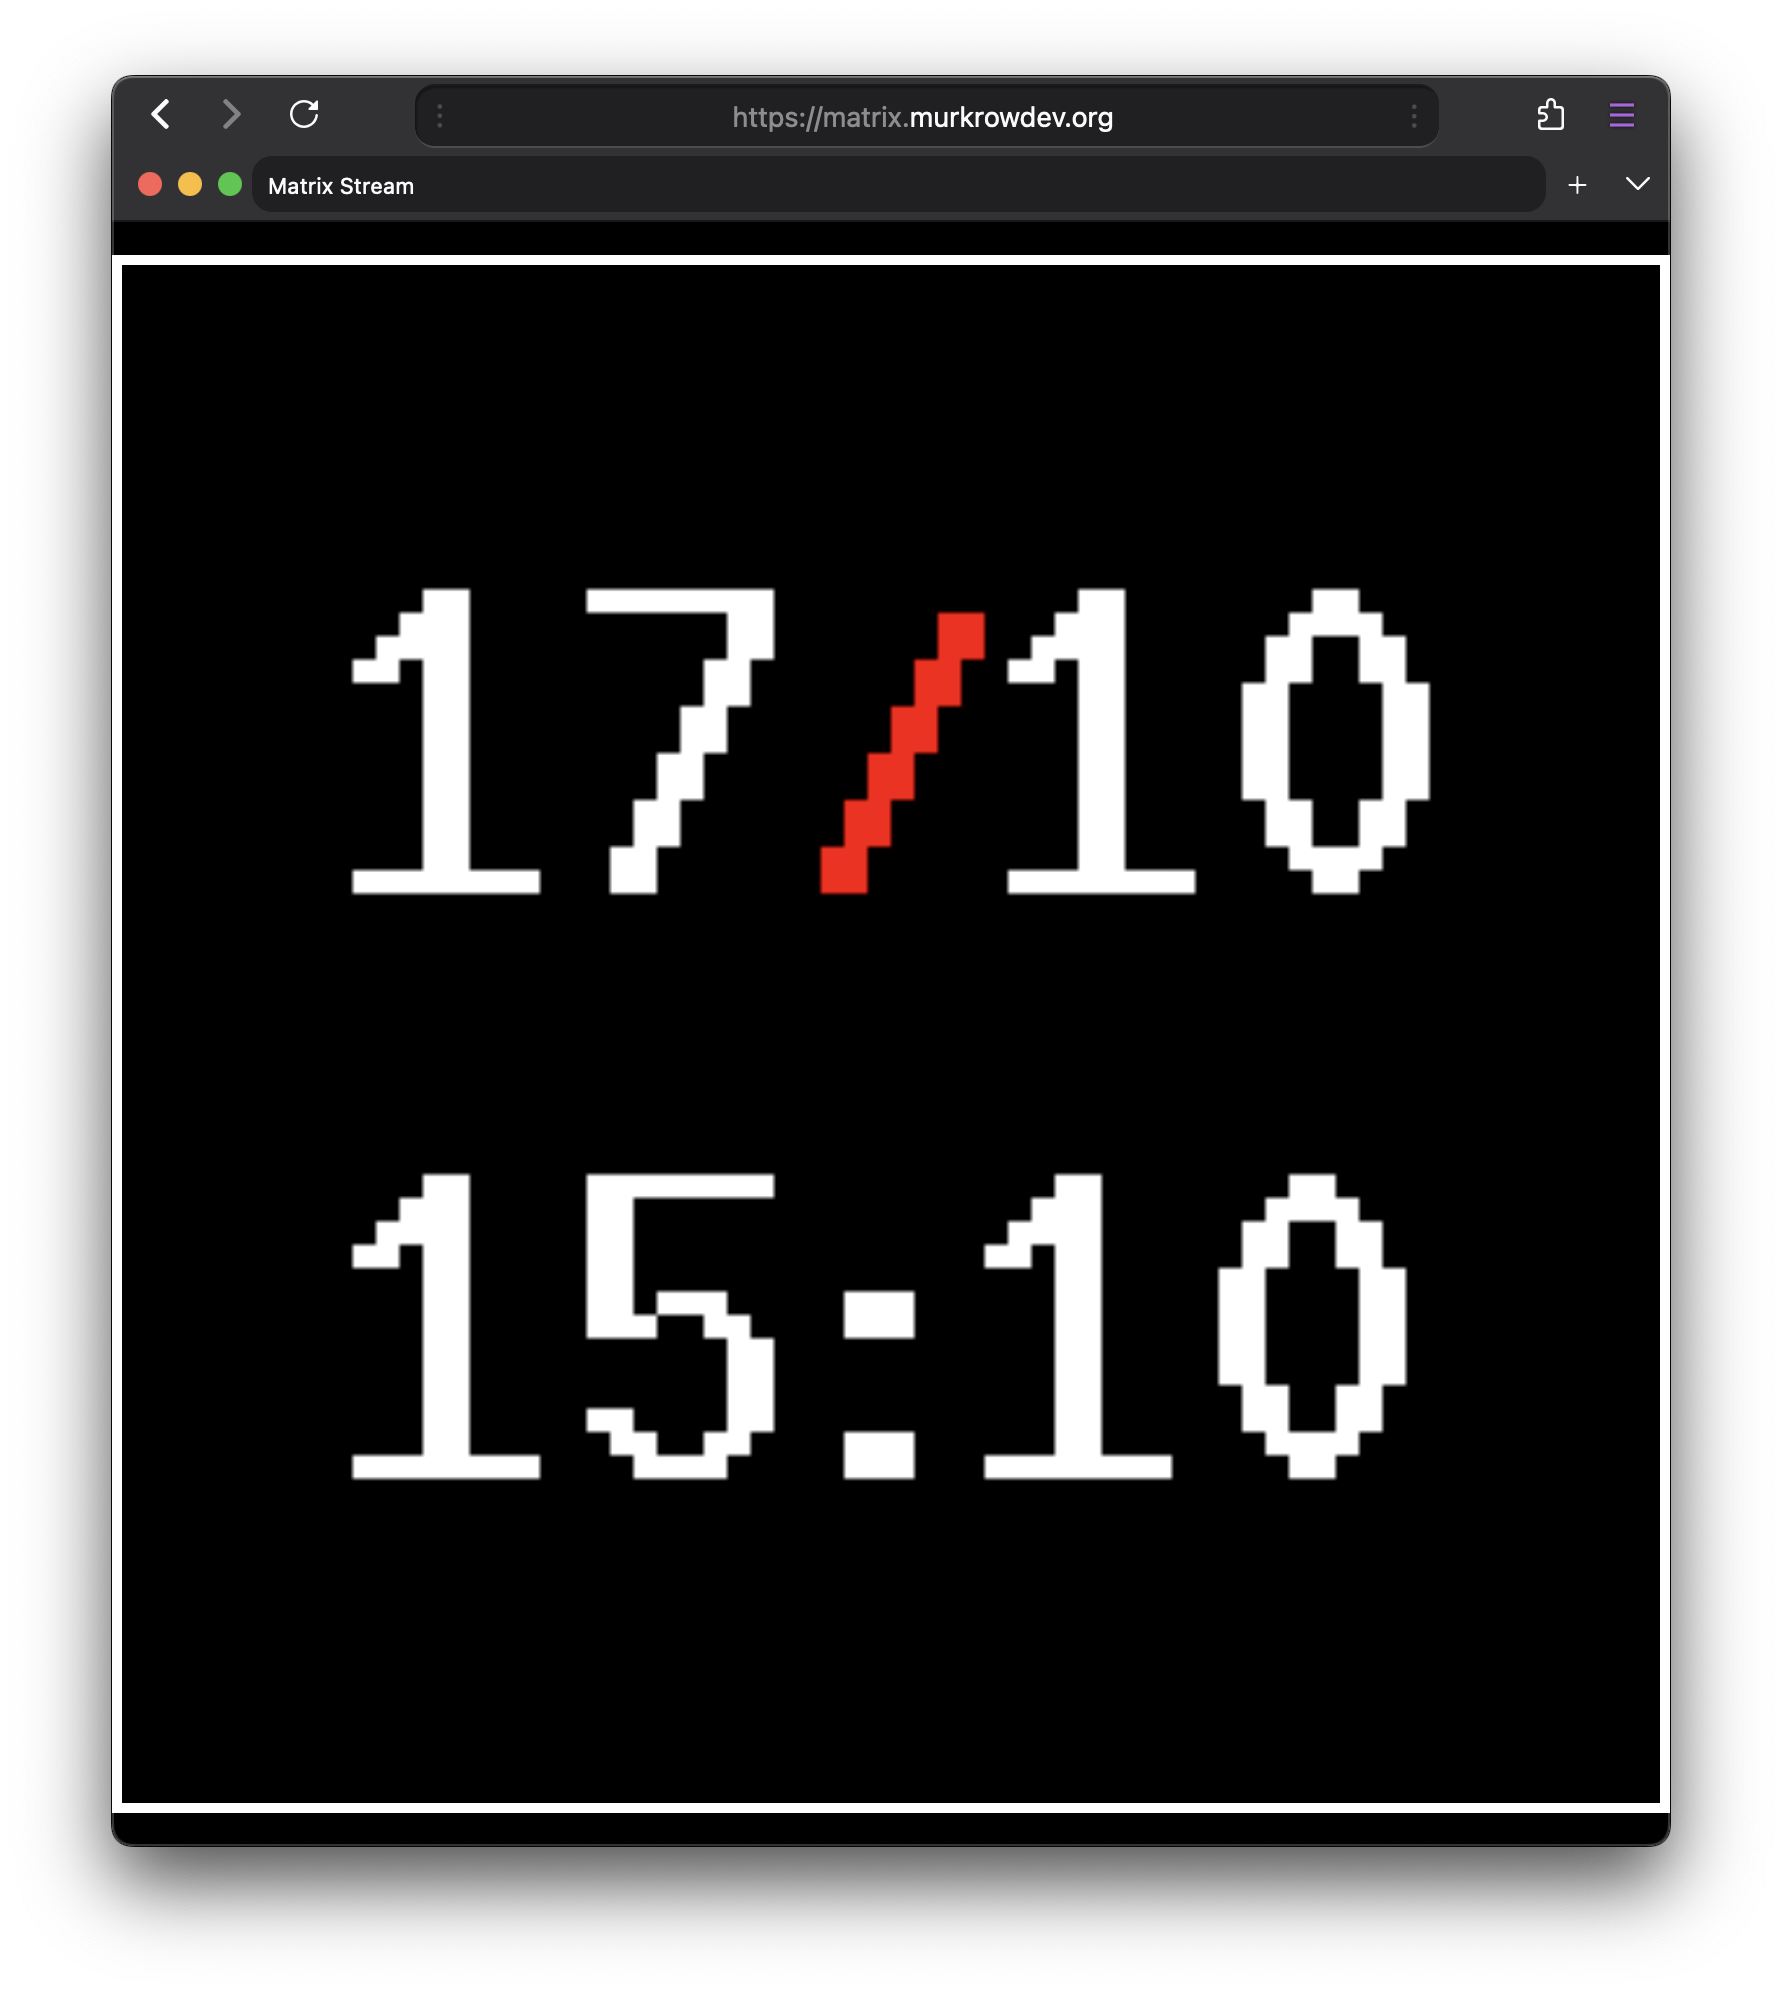
\includegraphics[width=\textwidth]{tesi/img/matrices/web.png}
    \caption*{Web simulator}
\end{minipage}
    \centering
    \begin{minipage}[b]{0.32\textwidth}
        \centering
        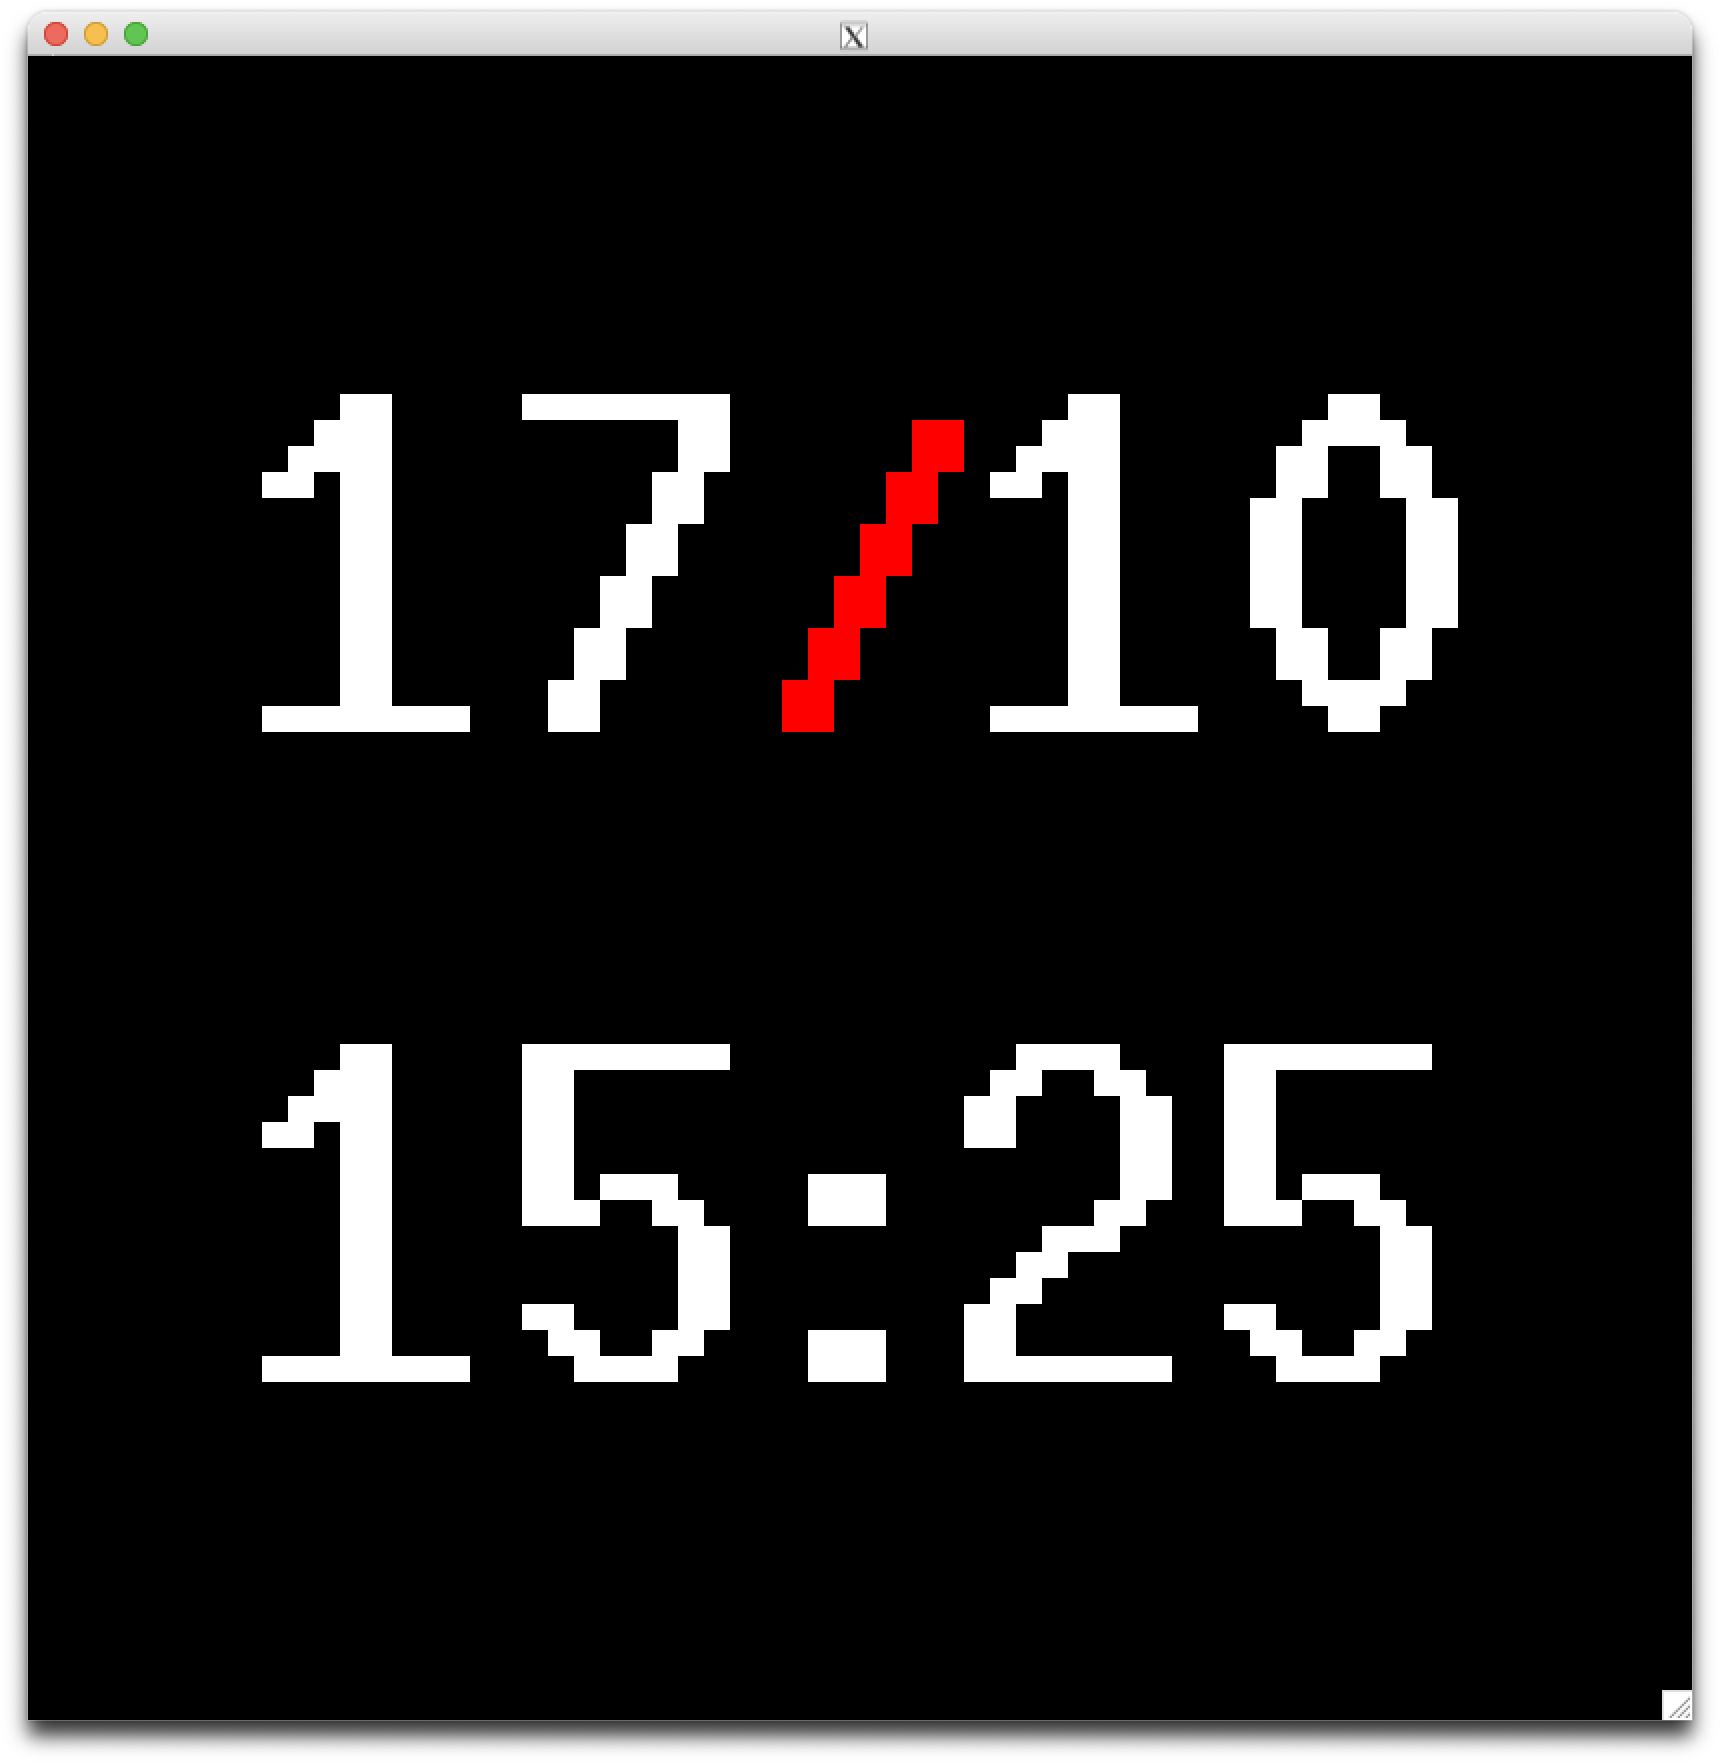
\includegraphics[width=\textwidth]{tesi/img/matrices/x11.png}
        \caption*{X11 windowed simulator} 
    \end{minipage}
    \centering
    \begin{minipage}[b]{0.32\textwidth}
        \centering
        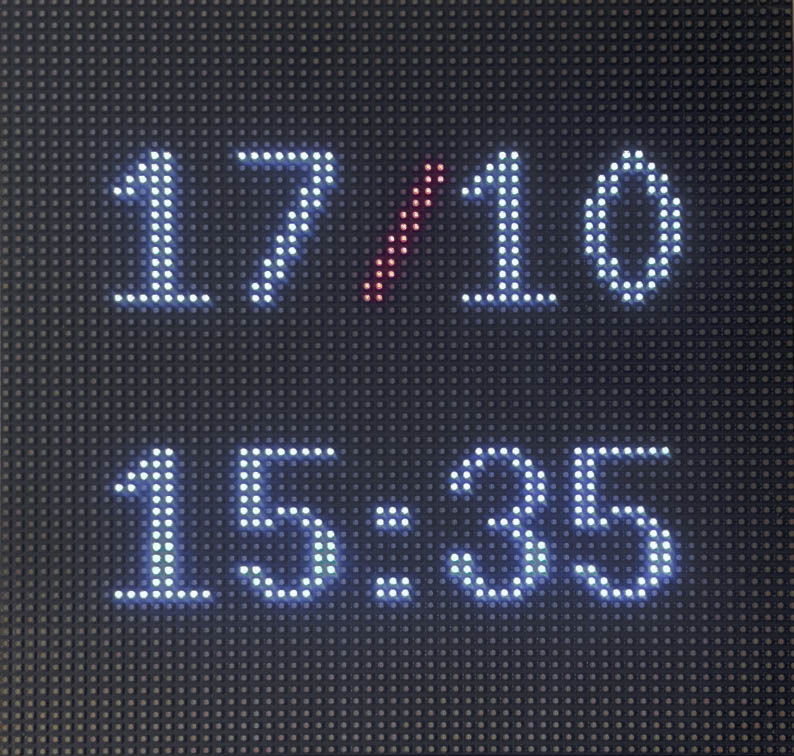
\includegraphics[width=\textwidth]{tesi/img/matrices/real.jpg}
        \caption*{Real matrix} 
    \end{minipage}
\end{figure}


Even with cross-compilers meticulously configured, the process of compiling and syncing files continued to be a significant drain on development time. Furthermore, given that I am frequently away from home, I sought a solution that would allow me to work on the project remotely, without the need for the physical hardware. Clearly, carrying the matrix and Raspberry Pi with me at all times was not a practical option. This led me to explore the idea of developing a matrix simulator from scratch.

Initially, the task appeared daunting, as I anticipated that a substantial amount of time and effort would be required to implement such a simulator. However, once again, the design principles employed throughout the application—particularly the use of dependency inversion—proved to be immensely beneficial.

One of the key architectural decisions in the project was to ensure that, aside from the application’s entry point, no other modules would have direct knowledge of the matrix hardware. Instead, all modules interact with a generalized abstraction—a \textit{Canvas} interface. This meant that, in order to implement the simulator, I only needed to create a new class that conformed to the \textit{Canvas} interface, and dynamically switch between the actual hardware matrix and the simulator based on specific conditions.

These conditions were introduced through a pre-processor argument passed during the compilation process, enabling the system to determine whether to instantiate the actual hardware or the simulated matrix. Subsequently, I modified the main application logic to utilize a \textit{MatrixBuilder} class, which abstracts the creation of the matrix, making it agnostic to the specific implementation (hardware or simulation). The \textit{MatrixBuilder} class is a simple factory that returns a \textit{MatrixDevice} object, based on the conditions provided during compilation.

\begin{minted}{c++}
class MatrixBuilder
{
public:
    static MatrixDevice* build()
    {
#if SIMULATION
        return new X11Matrix();
#elif WEB
        return new MatrixStream();
#else
        return new HardwareMatrix();
#endif
    }
};
\end{minted}

The output of the \textit{MatrixBuilder} is a \textbf{MatrixDevice} object, which is a custom class I developed to encapsulate the various matrix implementations. This wrapping was necessary because the matrix class provided by the library could not be directly modified. Thus, I introduced a custom class to act as an intermediary, wrapping the existing library class.

\begin{minted}{c++}
class HardwareMatrix : public MatrixDevice {
private: RGBMatrix *matrix;
public: 
HardwareMatrix() {

    // Configure the RGBMatrix
    RGBMatrix::Options matrix_options;
    rgb_matrix::RuntimeOptions runtime_opt;

    // Create the RGBMatrix object
    RGBMatrix *matrix = RGBMatrix::CreateFromOptions(matrix_options, runtime_opt);
    this->matrix = matrix;
}
Canvas* CreateFrameCanvas()
{
    return matrix->CreateFrameCanvas();
}
void SwapFrameCanvas(Canvas *canvas){
    matrix->SwapOnVSync((FrameCanvas*)canvas);
}
}; \end{minted}

This design provided the necessary flexibility, allowing me to switch between different matrix implementations without significant modifications to the underlying logic. The use of a wrapper class ensured compatibility with the existing library while offering the opportunity to extend functionality when necessary.

\subsection{The X11 Simulator}

The X11-based simulator serves as a graphical approximation of the actual matrix hardware. By leveraging the X11 windowing system, it simulates the behavior of the matrix display in a window on the desktop environment, replicating the visual effects and behavior of the matrix as a 1:1 replica of the original. This is the actual simulator I used while developing the application since is the better performing one.

\subsection{The Web Simulator}
\label{web-simulator}
The web-based simulator provides a more accessible, platform-independent alternative, allowing users to interact with the system remotely. It is composed of two main components: a C++ module responsible for rendering frames, which serializes them as an array of RGB values and transmits them through a UNIX socket, and a Python server built with Flask. The Flask server receives the data, processes it, and transmits it in real-time via WebSockets to an HTML page, also served through Flask, where the live stream is rendered for users to interact with.

This design offers real-time simulation capabilities and enables users to experience the system without the need for physical hardware. A publicly accessible instance of this simulator has been deployed to allow users to test Mosaico, available at \url{https://matrix.murkrowdev.org/}.